\documentclass[aspectratio=1610, 13pt]{beamer}
\usepackage{xcolor}
\usepackage{multicol}
\usepackage{mathtools,array}
\usepackage[T1]{fontenc}

\usepackage{dutchcal}
\usepackage{zi4}
\usepackage[font={scriptsize,bf}]{caption}
% \usepackage{subcaption}
\usepackage{graphics}
\usepackage{tikz}
\usepackage{fontawesome5}
\usepackage{mathpartir}

\newcommand{\naturals}{\mathbb{N}}
\newcommand{\reals}{\mathbb{R}}

\newcommand{\Dist}[1]{\mathcal{D}(#1)}
\newcommand{\expectation}{\mathbb{E}}

\newcommand{\states}{S}
\newcommand{\actions}{A}
\newcommand{\observables}{O}
\newcommand{\trans}{T}
\newcommand{\obs}{Z}
\newcommand{\reward}{R}
\newcommand{\discount}{\gamma}

\newcommand{\beliefs}{\mathcal{B}}
\newcommand{\beliefUpdate}{\tau}

\newcommand{\policy}{\pi}

\newcommand{\diff}[1]{\mathop{}\!\mathrm{d}#1}
\renewcommand{\figurename}{Figure}
\renewcommand{\refname}{Reference}

\AtBeginDocument{
  \catcode`_=12
  \begingroup\lccode`~=`_
  \lowercase{\endgroup\let~}\sb
  \mathcode`_="8000
}

% \usetheme{Madrid}
% % \usetheme{default}
% \setbeamertemplate{caption}[numbered]
% \setbeamerfont{title}{size=\large}
\mode<presentation>
{
  \usetheme{Darmstadt}      % or try Darmstadt, Madrid, Warsaw, ...
  \usecolortheme{default} % or try albatross, beaver, crane, ...
  \usefonttheme[onlymath]{serif}  % or try serif, structurebold, ...
  \setbeamertemplate{navigation symbols}{}
  \setbeamertemplate{caption}[numbered]
  \setbeamertemplate{footline}[frame number] 
} 

\usepackage{listings}
\lstdefinestyle{heaplang}{
    language=Caml,
    basicstyle=\footnotesize\ttfamily,
    keywordstyle=\color{blue},
    commentstyle=\color{red},
    escapeinside={<@}{@>},
    morekeywords={new_chan, fork, recv, send, swap, ref}
}
\lstdefinestyle{clang}{
    language=Caml,
    basicstyle=\footnotesize\ttfamily,
    keywordstyle=\color{blue},
    commentstyle=\color{red},
    escapeinside={<@}{@>},
}
\lstset{style=heaplang}

\usepackage{natbib}

\newcommand{\buchi}{B\"uchi }

\definecolor{goldenpoppy}{rgb}{0.99, 0.76, 0.0}
\definecolor{goldenyellow}{rgb}{1.0, 0.87, 0.0}
\definecolor{green2}{rgb}{0.1,0.7,0.3} 
\newcommand{\gcheck}{{\color{green2}\faCheckCircle[regular] }}
\newcommand{\rcross}{{\color{red} \faTimesCircle[regular]} }
\newcommand{\rflag}{{\color{red} \faFlag}}
% \usepackage{algorithm,amsmath}
% \usepackage[noend]{algpseudocode}

\newcommand{\zlstinline}{\let\par\endgraf\lstinline}
\newcommand{\comments}[1]{{\color{red}#1}}
\title{Chapter 6: Algorithms}
\author{Reporter:  Xie Li}
\date{\today}
\begin{document}
\maketitle

\begin{frame}{Overview}
\begin{itemize}
\item [6.1] Worklist algorithm.
\item [A.C] Preliminaries.
\item [6.2] Iterating in reverse postorder.
\item [6.3] Iterating through strong components.
\end{itemize}
\end{frame}

\begin{frame}{Worklist Algorithm: Reaching Definition Analysis Example}

\begin{center}
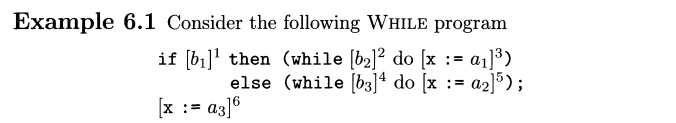
\includegraphics[scale=0.4]{rdexp.png}

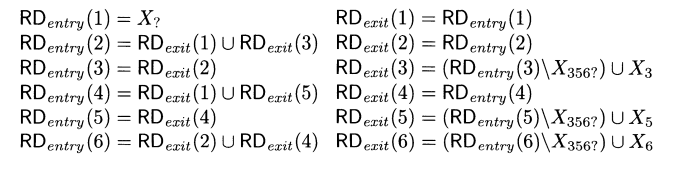
\includegraphics[scale=0.4]{rdexp1.png}
\end{center}

\begin{center}
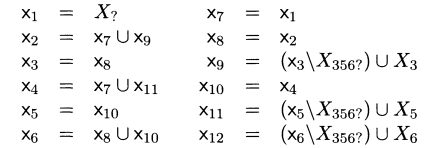
\includegraphics[scale=0.4]{rdexp2.png}
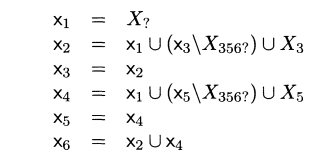
\includegraphics[scale=0.4]{rdexp3.png}
\end{center}

where $\mathbf{X}_{356?}$ represents $\{(x, 3), (x, 5), (x, 6), (x, ?)\}$

\end{frame}


\begin{frame}{Assumptions}
\begin{itemize}
\item 
\item 
\item 
\end{itemize}
\end{frame}


\end{document}